\chapter{Hybrid Eulerian-Lagrangian Vortex Particle Method}
\label{ch:helvpm}

% Summarize the sections. : domain decomposition, coordinate systems assosciated to each
% subdomains, and the coupled evolution of the hybrid method.
% Reference to the literatures: Cottet and others, stock and daenick
% We use approach of stock based on the phd research of daeninck

	\section{Introduction to Hybrid Eulerian-Lagrangian Vortex Particle Method}
	
	The \printAcron{Hybrid Eulerian-Lagrangian Vortex Particle Method}{HELVPM} is a domain decomposition method, where the Eulerian method and the Lagrangian method solve different regions of the fluid. The domain decomposition method simply splits the domain of interest and uses the appropriate method in each domain. The Eulerian formulation will be used at the near-wall region, where we need proper description of the vorticity generation at the boundary, and the Lagrangian formulation is used away from the body, where we only need to evolve the vorticity field. Figure \ref{fig:domainDecomposition} shows the decomposition of the domain into the gridded and the non-gridded region.
	
		\begin{figure}[!h]
			\centering
			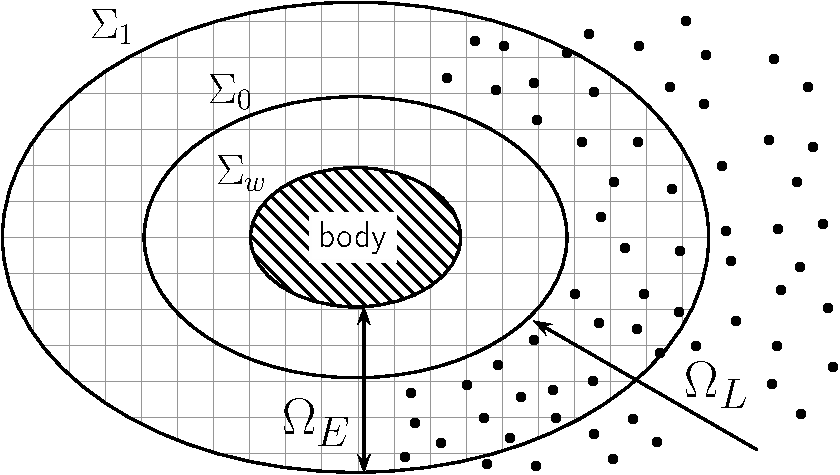
\includegraphics[width=0.6\linewidth]{figures/hybrid/domainDecomposition_typical_type2-crop.pdf}
			\caption{Standard domain decomposition using Schwartz iteration for coupling the two methods. Eulerian subdomain $\Omega_E$ (near the body), and Lagrangian subdomain $\Omega_L$ (away from the body). Figure is based on Guermond (2000) \cite{Guermond2000a}.}
			\label{fig:domainDecomposition}
		\end{figure}	
	
	Several studies have already been performed regarding the domain decomposition. Cottet and Koumoutsakos (2000a)\cite{Cottet2000a} summarized the theory behind the Eulerian-Lagrangian domain decomposition. Guermond and Lu (2000) \cite{Guermond2000a} simulated the advection dominated, external flows. They used Schwartz type method to couple the two methods together. Ould-Salhi et al. (2001) \cite{Ould-Salihi2001a} blended the finite difference and vortex method together to construct the hybrid method. Winckelmans et al. (2005a) \cite{Winckelmans2005} investigated the trailing vorticies. Daeninck (2006) \cite{Daeninck2006} used a simplified coupling strategy without the Schwartz method, to couple Vortex Particle Method and Finite Difference Method together. Stock (2010) \cite{Stock2010a} expanded Daeninck's strategy, coupling Vortex Particle Method and Finite Volume Method and modeled a 3D rotor.

	\section{Convectional Coupling Strategy}
	\label{sec:helvpm-ccs}
	
	When investigating the literature works, we see that not all domain decomposition methods are the same. The main difference between the methods is their coupling strategies. Most works employ the\textit{ Schwartz alternating method} to couple the vortex particle method and the grid solver. The Schwartz alternating method (or sometimes referred to as Schwartz iterative method), couples the vortex particle method and the grid solver by iteratively determining the boundary condition such that the stream functions in both domains, $\psi_L$ and $\psi_E$ in the Lagrangian domain $\Omega_L$ and the Eulerian domain $\Omega_E$ respectively, match at the overlap region $\Omega_E\cap\Omega_L$, shown in Figure \ref{fig:domainDecomposition}. The summary of a single iteration of the Schwartz alternating method is as follows:
	
		\begin{itemize}
		\item Determine the Eulerian boundary condition, the stream function $\psi_{\Sigma_1}$ at the Eulerian boundary $\Sigma_1$, extracted from the Lagrangian stream function $\psi_L$ in the Lagrangian subdomain $\Omega_L$.
		\item Solve for the stream function $\psi_E$ in the Eulerian subdomain $\Omega_E$ with the new boundary condition $\Sigma_1$.
		\item Determine the Lagrangian condition, the stream function $\psi_{\Sigma_0}$ at the Lagrangian boundary $\Sigma_0$, extracted from the Eulerian stream function $\psi_E$ in the Eulerian subdomain $\Omega_E$.
		\item Solve the stream function $\psi_L$ in the Lagrangian subdomain with the boundary conditions $\psi_{\Sigma_0}$ at the Lagrangian boundary $\Sigma_0$.
		\end{itemize}
	
	This procedure is iterated until the stream functions of both domains converge \cite{Ould-Salihi2001a}. Once the stream function is determined in both the domains, the velocity field can be obtained. Using the velocity field, we can then evolve the vorticity field in the Lagrangian subdomain.

	\section{Simplified Coupling Strategy}
	\label{sec:helvpm-scs}
	
	As we realized now, the downside to this procedure is that we have to solve the stream function in both $\Omega_E$ and $\Omega_L$ iteratively, until we converge to a solution. This makes the computation very expensive, especially when we are dealing with large numbers of vortex particles. Therefore for this project, we decided to use the coupling technique formulated by Daeninck (2006) \cite{Daeninck2006} and expanded by Stock (2010) \cite{Stock2010a}. However, through the course of the present work, we will see that we have to perform a modification to the scheme, to ensure that the total circulation of the Lagrangian domain is conserved at all times (see section \ref{seec:coupling-mthlcs}).	
	
%	\subsection{Coupling Eulerian and Lagrangian Methods}

		\begin{figure}[!h]
			\centering
			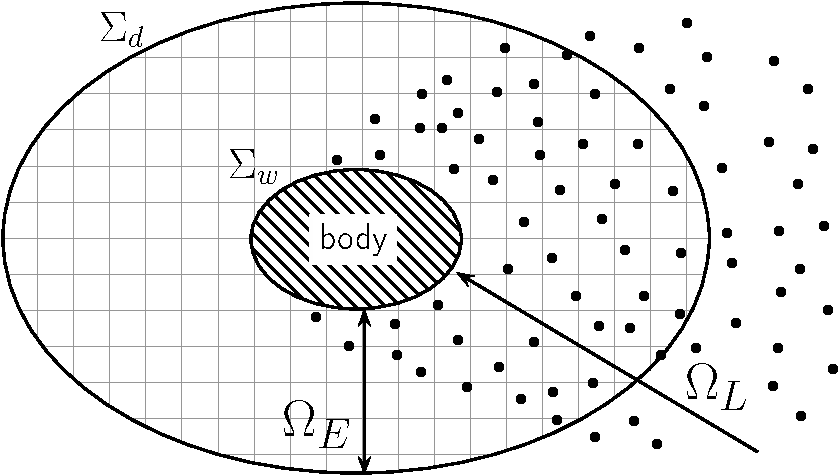
\includegraphics[width=0.6\linewidth]{figures/hybrid/domainDecomposition_daenick_type2-crop.pdf}
			\caption{Modified domain decomposition \underline{without} Schwartz alternating method. Lagrangian subdomain extends up to the surface of the body. Figure is based on Daeninck (2006) \cite{Daeninck2006}.}
			\label{fig:domainDecomposition_daenick}
		\end{figure}
	
	The simplified coupling strategy was first demonstrated in the doctoral thesis of Daeninck \cite{Daeninck2006}. Daeninck showed that it is possible to couple the Lagrangian and the Eulerian methods without the use of Schwartz iterative method. Daeninck proposed an approach that satisfies the following statements:
	
	\begin{itemize}
	\item The Lagrangian vortex method solves the full fluid domain $\Omega_L$ (see Figure \ref{fig:domainDecomposition_daenick}), but under-resolves the near-wall region $\Omega_E$ as it is less efficient at resolving the boundary layer of the flow.
	
	\item Eulerian method is used to resolve the near-wall region $\Omega_E$, efficiently capturing the boundary layer features and flow separation.
	
	\item The Lagrangian subdomain in the near-wall region $\Omega_L\cap\Omega_E$ is corrected using the more accurate Eulerian solutions to compensate the aforementioned under-resolution.
	
	\item The boundary conditions for the Eulerian method is directly obtained from the evolved solution of the Lagrangian method.
	\end{itemize}
	
	The grid solver therefore essentially acts as the correction for the under-resolved regions of the Lagrangian method. The Lagrangian vortex method in the full fluid domain focuses only on capturing and efficiently evolving the wake.
	
	Furthermore, the Lagrangian boundary condition is handled differently. Unlike the standard Lagrangian method, where the boundary sheds vorticity, in this strategy as the Lagrangian method is under-resolved at the boundary, it cannot be used to resolve the vorticity flux at the body. Instead, the Eulerian method is used to solve vorticity generation from the wall boundary, and acts as the vorticity generator for the Lagrangian method. For this coupling strategy to be valid, there are some assumptions that we must satisfy:

	\begin{itemize}
	\item At $t_n$ before the evolution of both methods to $t_{n+1}$, the Lagrangian solution matches the Eulerian solution at the boundary of the near-wall region $\Sigma_d$ (see Figure \ref{fig:domainDecomposition_daenick}).
	\item Even though the Lagrangian subdomain is under-resolved in the near-wall region, it should still be able to provide accurate boundary conditions for the Eulerian method at the external boundary $\Sigma_d$.
	\item After the evolution to $t_{n+1}$, the deviation of the Lagrangian solution (due to lack of vorticity flux at Lagrangian boundary), should be minimal.
	\end{itemize}	
	
	Daeninck's simplified coupling strategy focused on the vorticity-velocity formulation for the Eulerian domain. However, he briefly showed that it is also possible to couple the Eulerian method with the velocity-pressure formulation. The advantage of using the velocity-pressure formulation is that it will be easier to extend to a 3D problem, unlike the vorticity-velocity formulation for the Eulerian method.
	
	\subsection{Coupling Algorithm}	
	\label{subsec:hybrid-ca}
	The coupling of the solvers was described in one global time stepping algorithm. As the Eulerian methods suffers from a larger stability constraint on the time step, and the Lagrangian time marching is computationally more expensive, a  different time discretization for both methods was employed. The Lagrangian method and the Eulerian method had the time steps $\Delta t_L$ and $\Delta t_E=\Delta t_L/k_E$, respectively, where $k_E$ is the number of Eulerian substeps.
	
	Assuming that we known the solutions of both solvers at $t_n$, the algorithm for the coupled time marching of the Eulerian method (with velocity-pressure formulation) and the Lagrangian method from $t_n$ to $t_n+\Delta t_L$ is summarized as follows:
	
	\begin{enumerate}
	\item At $t_n$, \textbf{correct the Lagrangian solution} in the near-wall region $\Omega_L\cap\Omega_E$ from the Eulerian field, Figure \ref{fig:domainDecomposition_daenick}. The vorticity in $\Omega_E$ is determined by taking the curl of the velocity field of the Eulerian method. The vortex particles strengths are determined by interpolating the vorticity from the Eulerian grid.
	
	\item \textbf{Advance the Lagrangian method} from $t_n$ to $t_{n}+\Delta t_L$, with the corrected Lagrangian solution. However, after the correction there exists a slip velocity at the solid wall $\Sigma_w$. Therefore to properly evolve the solution, the Lagrangian method needs to enforce the \textit{no-slip} boundary condition at the wall. This is performed by computing the vortex sheet $\gamma$ that cancels this slip velocity at the wall. At the end of the evolution, classic vortex methods diffuse the computed vortex sheet to the particles but in hybrid case, it is performed by the Eulerian method.
	
	\item \textbf{Determine the Eulerian boundary conditions} for the velocity field $\mathbf{u}$ at $t_{n}+\Delta t_L$ from the evolved Lagrangian solution at $t_{n} + \Delta t_L$. The Eulerian method requires the Dirichlet velocity boundary condition at $\Sigma_d$ (the Eulerian Dirichlet velocity boundary) and the velocity boundary condition at the wall boundary $\Sigma_w$ for a velocity-pressure formulation is simply the zero slip velocity, Figure \ref{fig:domainDecomposition_daenick}.
	
		\begin{figure}[!t]
			\centering
			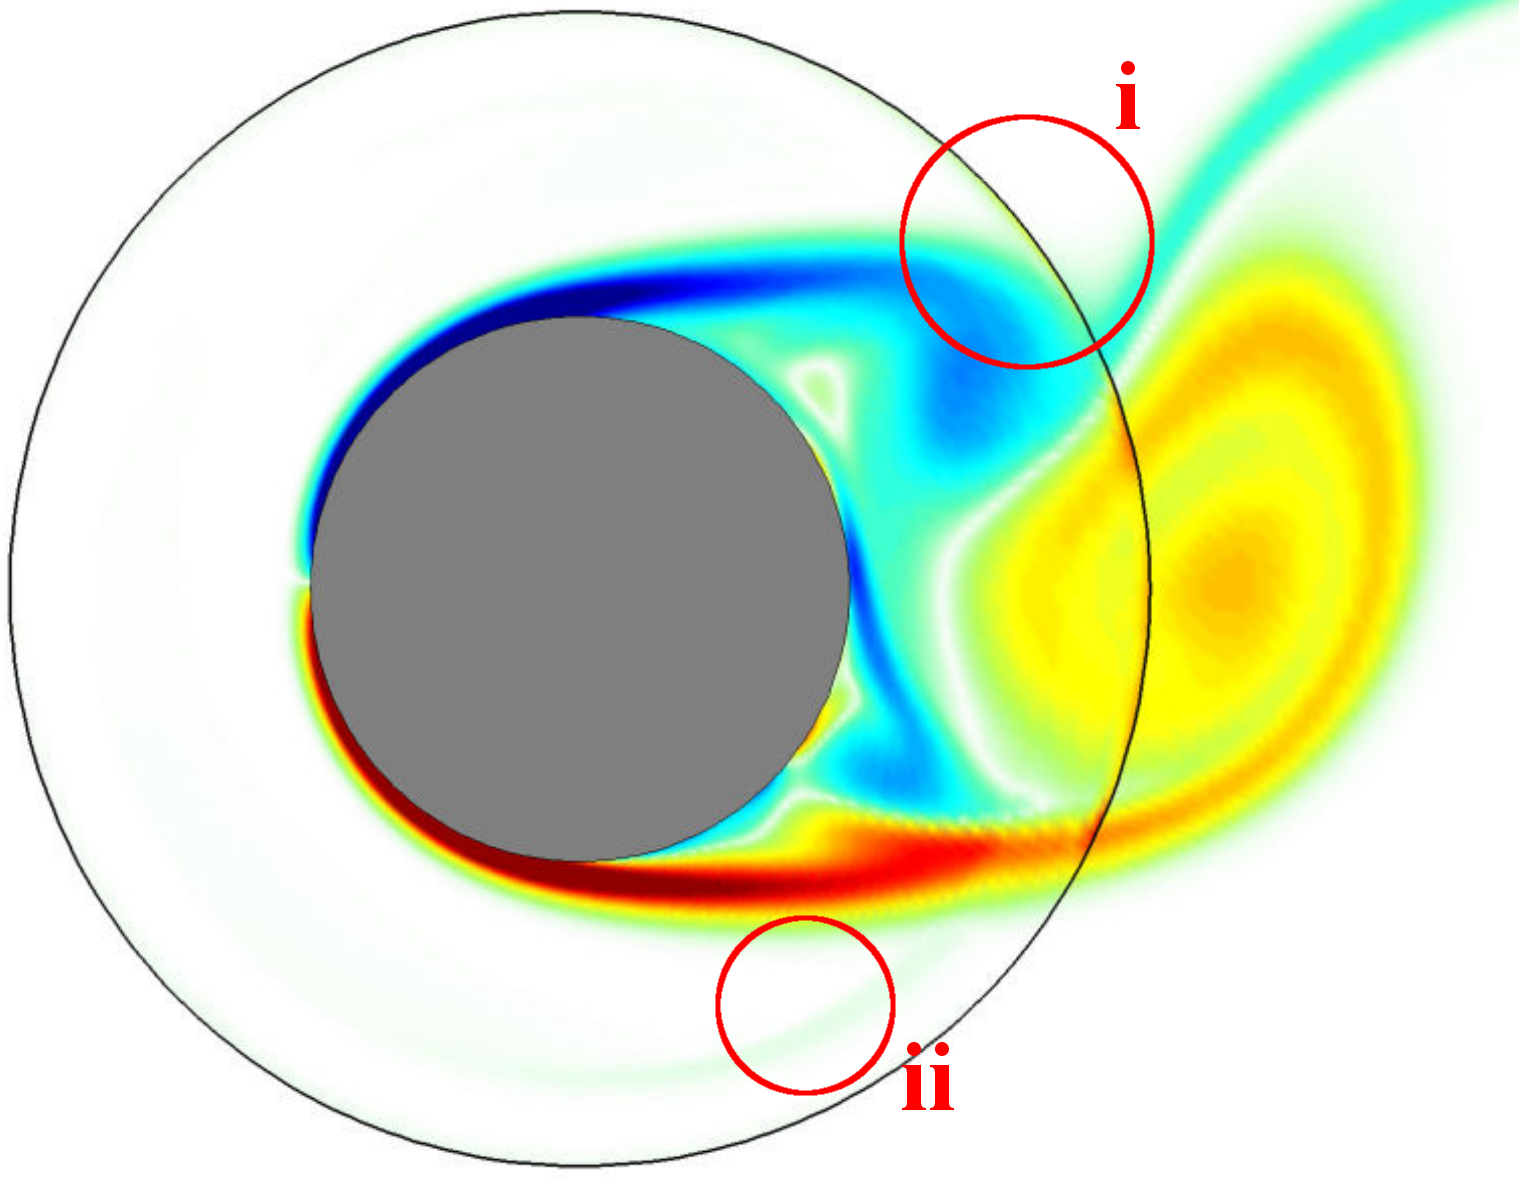
\includegraphics[width=0.5\linewidth]{figures/hybrid/daeninck_CylinderVorticityMod.png}
			\caption{Error at the transition from the Eulerian and the Lagrangian domain, obtained from Daeninck \cite{Daeninck2006}. The error is in the form of artificial vorticity at \textbf{i)} the Dirichlet boundary of the Eulerian domain $\Sigma_d$, and \textbf{ii)} the boundary of the Eulerian adjustment region shown in Figure \ref{fig:daeninckInterpolation}.}
			\label{fig:daeninck_CylinderVorticityMod}
		\end{figure}				
	
		\begin{figure}[!b]
			\centering
			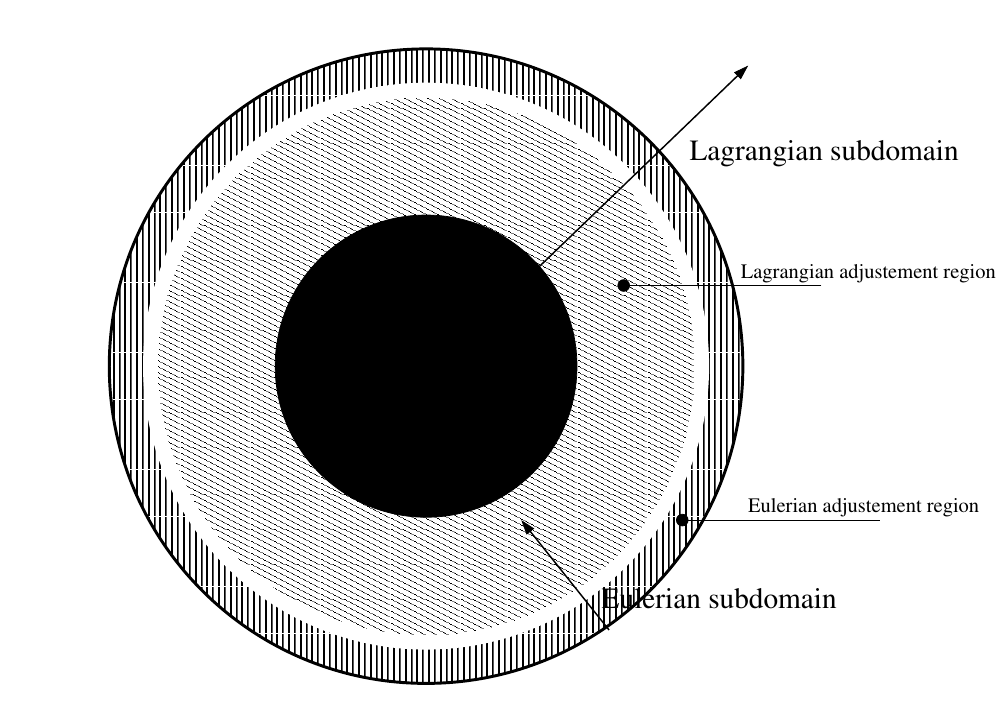
\includegraphics[width=0.5\linewidth]{figures/hybrid/daeninckInterpolationRegions.png}
			\caption{The domain decomposition and interpolation regions used by Daeninck \cite{Daeninck2006}. The outer Eulerian domain is also modified to enhance the coupling of the methods.}
			\label{fig:daeninckInterpolation}
		\end{figure}


	\item \textbf{Advance the Eulerian method} from $t_n$ to $t_n + \Delta t_L$ using $k_E$ Eulerian substeps. The boundary conditions on $\mathbf{u}$ at each substep is obtained by linear interpolation of the boundary condition at $t_n$ and $t_{n} + \Delta t_L$.
	\end{enumerate}	
	
	 Daeninck notices that when using the velocity-pressure formulation for the Eulerian method, the transition from the Eulerian to the Lagrangian domain is more noticeable. Figure \ref{fig:daeninck_CylinderVorticityMod}, shows the artificial vorticity at the boundary of the Eulerian domain $\Sigma_d$. This error is more prominent as the coupling is performed at the level of velocity, and we are looking at the curl of it, vorticity. To enhance the coupling of the Eulerian and the Lagrangian method, Daeninck further modified the Eulerian solution in the most external region of the Eulerian subdomain $\Omega_E$ interpolating the Lagrangian solution, and observed that it provided better results. Figure \ref{fig:daeninckInterpolation} shows the modified adjustments regions used by Daeninck in his work. 
 
	 However, in the present work we will use the Lagrangian correction strategy by Stock \cite{Stock2010a} and introduce additional modifications to the Lagrangian correction step itself to reduce this mismatch.
		
	
	\subsection{Lagrangian Correction Step}
	\label{subsec:hybrid-lcs}
	The coupling strategy demonstrated by Daeninck \cite{Daeninck2006}, was studied and was further extended by Stock \cite{Stock2010a}. Stock's work focused on the overlap region $\Omega_E\cap\Omega_L$ (Figure \ref{fig:domainDecomposition_daenick}) and correction of the Lagrangian solution. The following observations can be extracted from Stock's work:
	
	\begin{itemize}
	\item Eulerian solution is only assumed to be correct from the body surface $\Sigma_w$ to somewhat inside of the outer Eulerian domain $\Sigma_d$. Therefore, the transfer of the Eulerian solution to the Lagrangian method should take in account the potential inaccuracy of the Eulerian solution at the outer boundary (depicted in the results of Stock, Figure \ref{fig:stockBoundaryErrorMod}).
	
		\begin{figure}[!b]
			\centering
			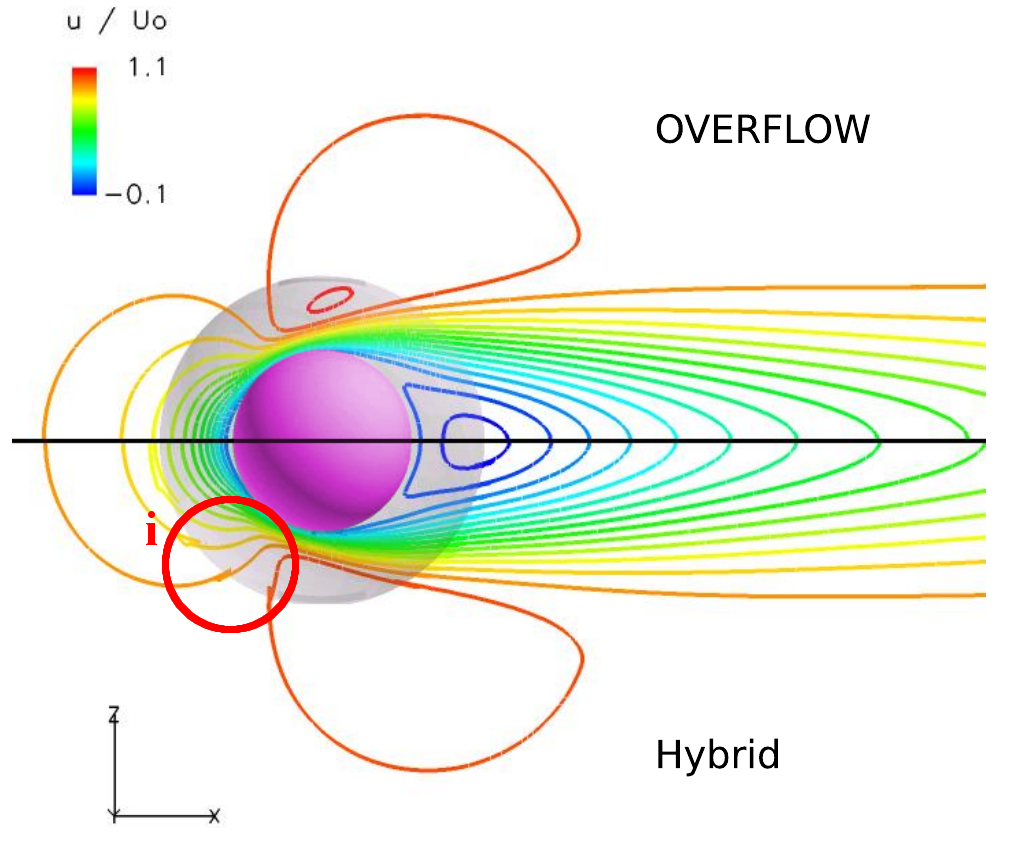
\includegraphics[width=0.5\linewidth]{figures/hybrid/stockBoundaryErrorMod.png}
			\caption{Mismatch in the Eulerian and the Lagrangian solution at the boundary $\Sigma_d$. The error is illustrated as \textbf{i)} slight mismatch in the velocity contours at the boundary.}
			\label{fig:stockBoundaryErrorMod}
		\end{figure}		
	
	\item The very strong gradient in vorticity (vortex sheet) cannot be efficiently and accurately transfered to the Lagrangian method. This is especially problematic at high Reynolds number flows, and interpolating this vorticity from the Eulerian method to the Lagrangian method results in numerical problems. Therefore, to avoid the noise in the interpolation, the correction step has to ignore the region very near to the wall.
	\end{itemize}
	
	The resulting Lagrangian correction domain, or the interpolation domain $\Omega_I$, using Stock's coupling approach, is shown in Figure \ref{fig:interpolationDomainDefinition}. If the Eulerian domain $\Omega_E$ is defined by $\partial\Omega_E=\Sigma_w \cup \Sigma_d$, then the interpolation region $\Omega_I$ is defined by $\partial\Omega_I = \Sigma_{i}\cup\Sigma_{o}$. The outer boundary of the interpolation domain $\Sigma_o$ is defined with an offset $d_{bdry}$ from the Eulerian Dirichlet velocity boundary $\Sigma_d$, such that potential inaccuracy of the Eulerian solution is ignored (depicted in Figure \ref{fig:interpolationDomainCloseup}). Similarly, the inner boundary of the interpolation domain $\Sigma_i$ is defined with an offset $d_{surf}$ from the Eulerian wall boundary $\Sigma_w$ such that the very strong vorticity (i.e the vortex sheet) is ignored (depicted in Figure \ref{fig:interpolationDomainCloseup}). The offsets $d_{surf}$ and $d_{bdry}$ were defined in the order of the Lagrangian vortex particle size.
	
	\begin{figure}[!t]
        \centering
        \begin{subfigure}[b]{0.45\textwidth}
                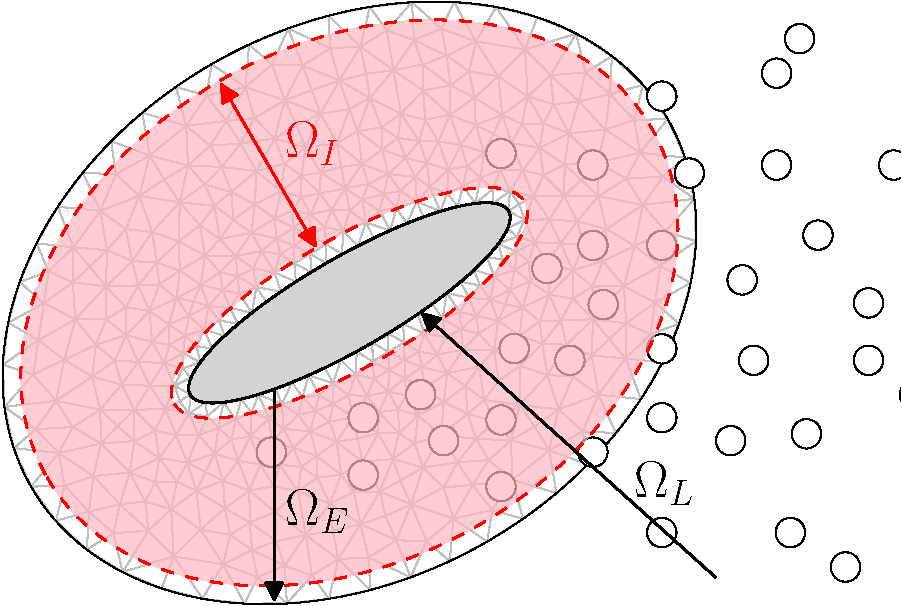
\includegraphics[width=\textwidth]{figures/hybrid/interpolationDomain/interpolationDomainExpanded-crop.pdf}
                \caption{Definition of the Domains}
                \label{fig:interpolationDomainExpanded}
        \end{subfigure}%
        \qquad %add desired spacing between images, e. g. ~, \quad, \qquad etc.
          %(or a blank line to force the subfigure onto a new line)
        \begin{subfigure}[b]{0.45\textwidth}
                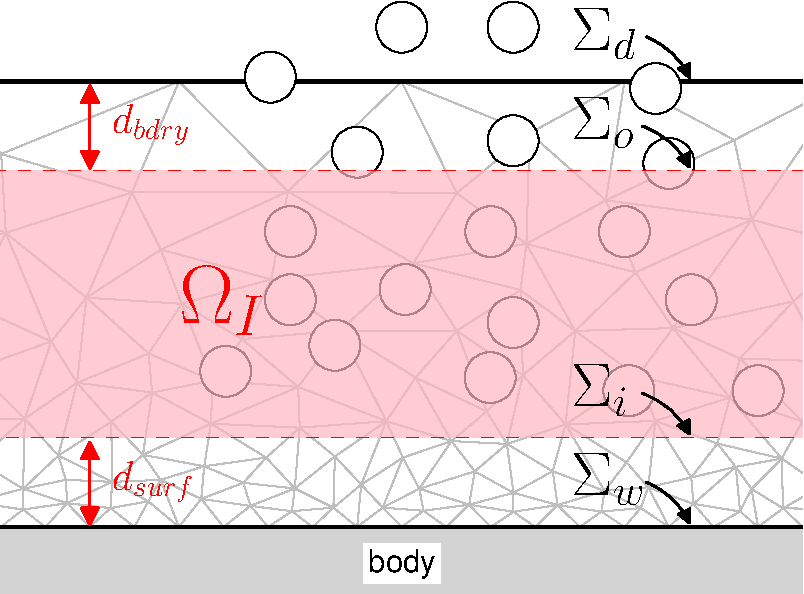
\includegraphics[width=\textwidth]{figures/hybrid/interpolationDomain/interpolationDomainCloseup-crop.pdf}
                \caption{Definition of the boundaries}
                \label{fig:interpolationDomainCloseup}
        \end{subfigure}
        \caption{Definition of the interpolation domain $\Omega_{int}$ for correcting the Lagrangian solution, with boundaries $\Omega_I: \partial\Omega_I=\Sigma_{i}\cup\Sigma_{o}$.}
        \label{fig:interpolationDomainDefinition}
	\end{figure}		

	The resulting Lagrangian correction step employed by Stock is summarized as follows:
	
	\begin{enumerate}
	\item Interpolate the vorticity of the Eulerian method from a non-uniformly structured (or an unstructured grid) onto a temporary uniformly structured Cartesian grid covering the entire Eulerian domain $\Omega_E$. This is done to performed an easier transfer of the Eulerian solution to the Lagrangian domain. The interpolation ignores the very strong vorticity present in the boundary layer that would otherwise cause numerical problem.
	
	\item Identify all the particles that are within the interpolation domain $\Omega_I$. These particles will be ones that is corrected.
	
	\item Correct or reset the strengths of the particles using the local particle area and the vorticity interpolated from the temporary structured Cartesian grid.
	\end{enumerate}
	
	Using this approach, Stock demonstrated the feasibility of simulating a 3D compressible flow problem around a sphere at $Re=100$, a finite airfoil at $Re=\num{1.5e6}$, and 4-Bladed advancing rotor at $Re=865,500$.
	
	\section{Evolution of the Hybrid Method}

	In the present work, we will therefore employ Daeninck's simplified coupling strategy with the detailed Lagrangian correction approach of Stock. The algorithm for the evolution of the hybrid method is divided into four key components:

	\begin{figure}[H]
		\centering
		\begin{tikzpicture}
			[node distance=.8cm, start chain=going below,]
			\node[punktchainN, join] (correct) {\textsf{Correct Lagrangian}};
		    \node[punktchainN, join] (evolveL) {\textsf{Evolve Lagrangian}};
		    \node[punktchainN, join] (bcE)     {\textsf{Determine Eulerian \\boundary conditions}};
		    \node[punktchainN, join] (evolveE) {\textsf{Evolve Eulerian}};
		\end{tikzpicture}
		\caption{Flowchart of the simple coupling strategy. The flowchart shows the procedure to evolve both methods from $t_n$ to $t_{n+1}$.}
		\label{fig:flowchart_simpleCoupling}
	\end{figure}

		\begin{enumerate}
		\item \textbf{Correct Lagrangian:} Use the solution of the Eulerian subdomain $\Omega_E$, to correct the solution of the Lagrangian subdomain $\Omega_L$, using the strategy of Stock (summarized in section 	\ref{subsec:hybrid-lcs}). Chapter \ref{ch:coupling} provides a detailed analysis on the implementation of Stock's Lagrangian correction strategy. Furthermore, the chapter highlights the limitations of Stock's correction strategy and described the methodology to ensure conservation of total circulation, paramount for a valid numerical scheme.
		
		\item \textbf{Evolve Lagrangian:} With the modified solution, evolve the Lagrangian solution from time step $t_n$ to $t_{n}+\Delta t_L$. Chapter \ref{ch:lagrangian} provides the detailed investigation on the theory and the algorithm used to evolve the Lagrangian solution.
		
		\item \textbf{Determine Eulerian boundary conditions:} Use the Lagrangian solution of time $t_{n}+\Delta t_L$ to determine the boundary conditions of the Eulerian subdomain at $t_{n}+\Delta t_L$. Chapter \ref{ch:coupling} describes the methodology used to determine the boundary conditions at each Eulerian substeps.
		
		\item \textbf{Evolve Eulerian:} With the boundary condition, evolve the Eulerian solution from $t_n$ to $t_{n}+\Delta t_L$ using $k_E$ Eulerian substeps. Chapter \ref{ch:eulerian} provides the detailed investigation on the theory and the algorithm of the Eulerian method used for the present work.
		\end{enumerate}
	
	Figure \ref{fig:flowchart_simpleCoupling} shows the flowchart of the evolution of the hybrid method. To ensure that the coupling of the hybrid method performs as explained in theory, we performed a verification and validation test on the functionality of each segregate methods.
	
%	\begin{figure}[!b]
%		\centering
%		\begin{tikzpicture}
%			[node distance=.8cm, start chain=going below,]
%			\node[punktchain, join] (correct) {Correct \\Lagrangian};
%		    \node[punktchain, join] (evolveL) {Evolve Lagrangian};
%		    \node[punktchain, join] (bcE)     {Determine \\Eulerian boundary conditions};
%		    \node[punktchain, join] (evolveE) {Evolve Eulerian};
%		\end{tikzpicture}
%		\caption{Flowchart of the simple coupling strategy. The flowchart shows the procedure to evolve both methods from $t_n$ to $t_{n+1}$.}
%		\label{fig:flowchart_simpleCoupling}
%	\end{figure}


	
	
